\chapter{Modeling} 
\label{cha:derivation}
%In diesem Kapitel kann das Modell vorgestellt werden, was erarbeitet oder bearbeitet wurde.
%%Purpose, Choice of NNs, Risk
This work's purpose is to investigate the statistical model of \glspl{ann} for its applicability to predicting important component temperatures inside \glspl{pmsm} in a field environment.
The distinctive feature with respect to other models established in this industrial field of research is training the model on empirical data exclusively without incorporating prior analytical knowledge from heat transfer theory.
As neural networks have been successfully applied to other sequence-to-sequence learning tasks (see sec. \ref{sec:ml_ann}) for both, regression and classification, chances are high to find this particular model also performing competitively for this thesis' underlying task.
The pending risk lays in the experimental data not being coherent enough between the input and the target data for any statistical model to find a suitable mapping and, secondly, in the model's possibly insufficient expressive capabilities.

%%Framework
Programming the whole framework for training neural networks is outside the scope of this work, all the more in view of the various existing frameworks already supported in different programming languages.
It was taken care in picking the most appropriate toolbox providing flexibility and adequate features.

%Feature engineering
Much effort was put into feature engineering, since this is a factor often determining the machine learner's success \cite{Domingo2012}.
Another reason is the fact, that, while models are of general purpose, features being inherent in training data are heavily domain-specific.
Though \glspl{ann} are known for being able to learn important features from data without having to design them explicitly, this is only prevalent for approximately infinite training examples.
Having a limited amount of empirical data, which is always the case in real-world applications and especially in this work, it is highly recommended to enrich the given data in order to make learning more effective. 

%Cross validation
For the evaluation of the different types of neural networks considered in this work, the training-validation-test subset separation was conducted.
More precisely, there are mutually exclusive subsets cut off the whole available experimental data and assigned to each the three different purposes.
Despite a possibly less biased evaluation rate through k-fold cross validation, the three sets are set constant.
This decision originates from having more computational throughput and, moreover, having comprehensive training data sequences generated from obviously different operation points.
The latter is also the reason, why hand-engineered separation of the data can exhibit fair distribution of operating characteristics over the subsets.
 
%%Regularization
As for any machine learner, generalization to unseen data is what counts.
Thus, there are concerns regarding \textit{over-fitting} and \textit{under-fitting}.
The former describes the process of learning the training data ``by heart'' and missing to learn to generalize to new data, which is expressed by high performance on training data and low performance on the unseen validation or test data.
Under-fitting, on the other hand, happens when the model is not classifying data better than random guessing or, in connection with continuous targets, when it is predicting data insufficiently. 

%% Hyper parameter optimization
Training a machine learning model is rife with hyper-parameters.
While selecting the weight parameters of a neural network via error backpropagation is considered as the first level of inference in model selection, the careful choice of those parameters determining the size of the neural network, the specific optimization technique or the precise weight initialization strategy etc. is called the second level of inference.
Most researchers opt for those parameters' intervals manually by trial and error (with significant success).
However, this work follows a more automated and constructive way of selecting hyper-parameters by the use of \gls{pso}.
Notice that the third level of inference, that is selecting the parameters of the \gls{pso}, is precluded from optimization and a meta-heuristic is applied instead. 

%%Gliederung
%The first section treats the question of which programming framework to choose, see section \ref{sec:framework}.
%After that, the several preprocessing techniques and means to enriching the training data are described in section \ref{sec:features}.
%A detailed outline of the evaluating cross validation is given in \ref{sec:cv}.
%Thorough explanations to the considered architectures and their mathematical background are outlined in \ref{sec:arch}.
%Optimization, weight initialization and regularization are hyper-parameters offering a variety of choices and are highlighted in sections \ref{sec:opt}, \ref{sec:init} and \ref{sec:reg}, respectively.
%The overall model selection strategy, namely the \gls{pso}, is embraced finally in section \ref{sec:pso}.
%
\section{Programming Framework}
\label{sec:framework}
Deciding for a framework one can choose from several options, each having its own characteristics. 
Among the most popular there are \textit{Caffe}, \textit{TensorFlow}, \textit{Theano} and \textit{Torch} (see \cite{BaRa2015} for a comparative survey).
This work builds upon the next-generation deep learning framework \textit{Chainer} \cite{Chainer2015}, which was developed for the Python programming language.
It is conveniently flexible and represents a standalone open-source tool providing simple and efficient methods for implementing sophisticated algorithms, training neural networks and adjusting parameters as well as hyper-parameters.
In contrast to other long-established frameworks, Chainer was designed with the necessity of versatile topologies and easy developing via standard programming language debuggers in mind.
Furthermore, Chainer provides automatic parallelization on CPUs and and near-to-automatic parallelization on GPUs.
Having chosen the Chainer framework for training models, the other required processes such as data loading, preprocessing, evaluation etc. are written in Python, consequently. 

Despite the well established numerical software MATLAB being an often applied tool for simulation and numerical analysis; and despite its use for the collection of the underlying benchmark data, its shortcomings for training \glspl{ann} are obvious in terms of open-source and flexibility.
MATLAB indeed provides a toolbox for neural networks, but its features are limited and do not reach the sophisticated level and the adaptability of the before mentioned frameworks. 

\section{Preprocessing and Feature Engineering}
\label{sec:features}
The data, which represents this work's investigative base, was gathered on a test bench having a three-phase \gls{pmsm} mounted with eight pole pairs.
The sample frequency was set to half a second consistently throughout the entire measurement. 
All parameters were received via first-order time-delay elements and a delay time $T_n$ of \SI{1.5}{\second}.

Besides mere thermal heat-up processes, which are not of much benefit for the training success, there is a total of 11 load profiles (with a dc-link voltage of \SI{250}{\volt}), each comprehensively measured and recorded during different operation points.
Each profile consists of the same set of recorded parameters.
Though there are plenty of variables, only 13 of them are of significant importance, as some are redundant with respect to others or simply not available outside the test bench setup.
Tab. \ref{tab:params} summarizes the parameters taken into account.
\begin{table}
	\caption{Considered input and target parameters. Note, that the dc-link voltage $u_{dc}$ as input quantity is omitted, because it is not utilized in the experiments, although it would be indispensable for an eligible application in the real world.}
	\label{tab:params}
	\centering
	\begin{tabular}{l c c}
		\toprule
		parameter name & symbol & model position \\
		\midrule
		ambient temperature & $\vartheta_a$ & input \\
		liquid coolant temperature & $\vartheta_c$ & input \\
		actual voltage $d$-axis component & $u_d$ & input \\
		actual voltage $q$-axis component & $u_q$ & input \\
		actual current $d$-axis component & $i_d$ & input \\
		actual current $q$-axis component & $i_q$ & input \\
		motor speed & $n_{mech}$ & input \\
		actual torque & $T_x$ & input \\
		\hline
		permanent magnet temperature & $\vartheta_{PM}$ & output \\
		stator teeth temperature & $\vartheta_{ST}$ & output \\
		stator winding temperature & $\vartheta_{SW}$ & output \\
		stator yoke temperature & $\vartheta_{SY}$ & output\\
		\bottomrule
	 \end{tabular}
\end{table}
As a consequence, every load profile holds altogether 12 sequences, one for each parameter.
Furthermore, each profile lasts for a different period of time, the shortest for around \SI{65}{\minute} and the longest for approximately \SI{366}{\minute}, which corresponds to sequence lengths of 7887 time steps and 43971 time steps, respectively.

It is important to point out, that the considered input quantities will be directly accessible on a real-world field application whereas all four output parameters will not be measurable.
Consequently, a trained model on the field would try its best to estimate the target quantities yet without knowing how well it is performing.

% discrepancy Soll Ist
Though the corresponding target performances of each actual input quantity is available as well, they can be considered redundant, since their dynamics are much higher than the sampling frequency and, thus, they do not provide a gain of information in comparison to the actual values.
% dc-link voltage u_dc
An important quantity is represented by the dc-link voltage $u_{dc}$, not depicted in tab. \ref{tab:params}, that is near to constant on either \SI{250}{\volt} or \SI{330}{\volt}, regarding the current operation mode.
Those with the lower dc-link voltage are investigated as a first step and the incorporation of those with the higher voltage are subject to future work.
% Approx. PM target
The permanent magnet temperature is approximated by the mean of four different sensors around the magnet's surface rather than measured directly from the core, in order to not diminish the magnets functionality for the motor.

%The data and its characteristics.

\subsection{Normalization}
As mentioned before, normalization of the data on its own is theoretically not mandatory when training neural networks.
Nonetheless, the amount of training examples is sparse and the parameters' scales differ vastly due to their different units (Kelvin, Volt, Nm etc.).
Hence, training would be dominated by one or two input quantities making training inefficient.
Moreover, as soon as activation functions like sigmoid or tanh are included, too large activations feeding the neuron would lead the mapping to be conducted on the saturating plateaus of these activation functions and hinder training enormously.
Gradients would shrink to near-zero values and, eventually, cause numerical problems stalling training.
Therefore, normalizing the data becomes inevitable for this thesis' particular task.

In this work, a simple normalization scheme is conducted.
If $x^{(t)}$ denotes the true value of a parameter $X$ to the time $t$ and $\bar{x} = \mu(X) = \frac{1}{N}\sum\nolimits_{t, i} x^{(t)}_i$ represents the sample mean of this parameter over each considered profile $i\in I$ while the parameters' unbiased sample standard deviation is computed by $\sigma(X)=\sqrt{(N-1)^{-1}\sum\nolimits_{t, i} (x^{(t)}_i - \bar{x})^2}$, then the normalized value $x_{norm}$ is calculated by  
\begin{align}
	x_{norm}^{(t)} = \frac{x^{(t)}-\bar{x}}{\sigma(X)}
\end{align}

Unfortunately, inherent with the normalization is the scenario in which a trained neural network would predict each normalized target equally well, but after undoing normalization there are mixed results due to the different standard deviations for each target.
As a remedy, one could design multiple models, one for each target, or build distinctive feed-forward nets on top of the recurrent topology in order to provide explicitly trainable structures accounting for the different targets' scales.
However, the latter approach would require more sophisticated target normalization.

\subsubsection{Removing Outliers}
% redundancy and outliers (see source code in DataPack.class)
Since the given data is physically measured, measurement errors such as unrealistic outliers may occur and need to be eliminated during a one-time preprocessing step.
There are outliers recurring especially in the beginning of each profile for specific parameters.
The pathological sequence holding these outliers constitutes a length of 10 to 15 time steps on average.

In order to remove them, a rectified window is slided through each sequence for every parameter.
Each data point is compared with the whole window's content.
If the value subtracted from the window's sample mean has an absolute value higher than three times the window's sample standard deviation, it is marked as outlier.
Upon detection, each outlier is replaced by the window's sample median.
A window size of 40 time steps has been found to accurately detect all outliers and simultaneously does not harm valid values.

\subsubsection{Principal Component Analysis}
In a further attempt to ease learning, \gls{pca} can be applied to the data.
\gls{pca} is a method for diagonalizing data and is also applicable for linear dimensionality reduction \cite{Bishop2006}.

If each input/output parameter represents a dimension in the feature space, \gls{pca} would find a transformation of each data point onto those axes explaining most of the data in a descending order, while keeping these axes orthogonal to each other.
The axes, onto which data is projected, are called principal components and their orientation in the feature space is defined by the data's eigenvectors.
Since their alignment is orthogonal with respect to each other, the elements of a feature vector become uncorrelated.
The feature dimension could be reduced then by neglecting the last principal component, that is the eigenvector corresponding to the smallest eigenvalue of the data.
By repeating this procedure, most of the data's variance would be sustained until there is only one dimension explaining the most variance of the data explainable by one axis.

A typical application would be the reduction of the data's dimensionality such that at least 90 percent of the variance is preserved.
Anyhow, reducing the dimensionality is optional and the data's diagonalization alone may already expose essential characteristics for the learning algorithm.

\subsection{Data Enriching}
\label{ssec:data_enriching}
There are eight input parameters, as shown in tab. \ref{tab:params}, that are directly measured and describe features the model has to learn from to estimate the targets sufficiently.
Enriching the data with reasonable features is recommended \cite{Domingo2012} for the sake of learning success, especially if only limited training examples are available.
During designing additional features, one must consider which quantities are accessible on the field, and, especially in this work's context, how much prior knowledge (e.g. from heat transfer theory) is adequate before the frontiers of black-box modeling are surpassed.

\subsubsection{Additional Features}
As a first step, a few quantities are added, that are easily inferable from the current data at each time step.
Foremost, the simplest addition is the absolute current and voltage defined by their $dq$-components:
\begin{align}
	|U| = \sqrt{u_{d}^2 + u_{q}^2} \\
	|I| = \sqrt{i_{d}^2 + i_{q}^2}.
\end{align}
Another hand-designed quantity is the following term defined by the current $dq$-components, that has a loose relation to $\Psi$ \cite{LeVa2014}:
\begin{align}
	i_d - \frac{i_q^2}{i_d} \sim \Psi
\end{align}
These three extra variables are not measured but calculated from the actual time step and added to the model's input in hope of them coming to the aid of training.

The second addition of input variables is by means of the first statistical moment and the second central moment of the preceding data.
In contrast to the before mentioned self-added quantities, the benefit from past data information is more obvious, since time series are to be predicted.
Having predefined a number of preceding time steps that are taken into account, the model receives the sample mean and variance of every input parameter along this time window at every point in time.
That is an addition of at most 22 input sequences to the neural network, provided that there was no dimensionality reduction during preprocessing earlier.
The resulting improvements in training are significant and are discussed in detail in the next chapter.
Notice, that this method evokes the necessity of a new hyper-parameter, that is the length of the preceding sequence to be examined, which is subject to optimization.

Though the facilitation of past data leverages performance, it is worth to mention, that this method also elevates memory consumption, which unfortunately depicts a bottleneck in automotive applications.
For every time step more to be considered, there is a further input-sized amount of values to be kept in memory in order to be able to infer its statistical properties.
In consideration of the fact, that this work is conducted from an academic perspective and in view of the ever-growing memory capabilities in all industrial fields, there are indeed time windows incorporated in this work's experiments, that would not be feasible in a today's deployment.  
Nevertheless, they soon might be and are hence not neglected.

\subsubsection{Subsequences}
In other thoroughly investigated application fields incorporating \glspl{ann}, the amount of training examples is usually very high while the size of each training example is relatively small.
In computer vision, for instance, each training example is represented by a picture with a limited amount of pixels and the number of available pictures is often larger than it might be possible to train on in an adequate time period.
Notably, each training example is of the same size, that is the same number of pixels.
In automatic speech recognition, further, spoken sentences are the matter of interest, which though have not equal lengths yet seldom last for more than a bunch of seconds. 
Admittedly, those two areas of research constitute very different sorts of data as opposed to this thesis' underlying benchmark data being of tabular form.
Yet the typical proportion of training example size with respect to the amount of available data is obviously contrary to what is addressed in this work - 11 load profiles, each lasting for one or more hours.

Therefore, the very custom approach of breaking down the few available load profiles in a lot shorter subsequences of equal length is put into practice.
This is reasonable for plenty of vital advantages: first of all, training is significantly faster by combining several training examples into a mini-batch, where the mean over all examples serves for the gradient computation.
The bigger the batch size, the faster training examples are processed.
This so-called mini-batch training represents the state of the art, due to the immensely higher throughput of data caused by utilizing parallel computation through more efficient matrix multiplications.
It has been shown, that batch training (all training data in a single batch) necessitates more epochs before convergence \cite{WiRa2003}, but in case of mini-batches, this effect is far less harmful while there is still a fundamental speed-up.
The specific implementation of this kind of training in this work is covered in sec. \ref{ssec:add_strats}.

A second point in favor of subsequences is the fact, that memory consumption is lower, since shorter sequences are processed and thus less gradients are accumulated, that could lead to a memory overflow elsewise.
It becomes evident, that it is essential to find a suitable trade-off between comprehensive data sequence lengths and memory capabilities, moreover because too short sequences would lessen the model's chances to find latent patterns while too long sequences decrease the amount of training examples and also might bring training to an unexpected halt.    

As a consequence, the subsequence length is another hyper-parameter being subject to optimization.
Having defined a length, all subsequences will constitute this size.
That is also necessary for the implementation of more sophisticated topologies (see sec. \ref{sec:arch}).

Naturally, since it will never be the case, that all load profiles at once are divisible in whole numbers by any subsequence length, there are inevitably small remainders being shorter than the predefined length in most of the profiles that are not processable.
These smaller parts can - depending on the chosen length - comprise time steps explaining close to 50 percent of the whole profile in a worst case scenario.  
In order to mitigate this loss of training data, the subsequences selected from the whole training set are varied each epoch.
In particular, before each epoch, there is a random offset determined as of which subsequences are drawn from a profile.
This offset is at most as big as the longest theoretical remainder for that profile in terms of a modulo operation.
Hence, for each epoch there is indeed some data not considered for training, but it will not be the exactly same data every epoch, such that after enough iterations it is ensured, that the model has seen almost all possible training data.
Furthermore, by following this sort of data enriching, the model will receive slightly different subsequences over and over again.
This can be imagined as noise applied to the data, which is known to mitigate the problem of over-fitting. 
Fig. \ref{fig:subsequences} illustrates the break down into subsequences.
Trivially, the subsequence windows are equal along the parameters in order to preserve correspondence between them.
\begin{figure}
	\centering
	\def\svgwidth{0.8\columnwidth}
         \import{eps/modeling/out/}{subsequences.pdf_tex}
         \caption{A sample load profile broken down into two subsequences. Every epoch, the offset is adjusted randomly between zero and the maximum length as of which the two subsequences would cover the whole remaining data, that is more precisely, until there is no small remainder in the end of the whole time series left. }
	\label{fig:subsequences}
\end{figure}

One might argue that longer comprehensive sequences are superior to multiple shorter sequences as this would show more resemblance with a real world application, but the gains through less computational time outweigh the loss in comprehensive sequences.
%Division into subsequences.

\section{Cross Validation}
\label{sec:cv}
When it comes down to comparing trained neural networks by their generalization ability, an ubiquitous measure of quality is required.
A recommended way of evaluating a machine learning model's performance, given a data set, is by \textit{k-fold cross validation}.
That is dividing the whole available set into $k$ subparts, leaving one part out for cross validation while training the model on the other $k-1$ data portions.
Repeating the hold out for each of the $k$ portions, one eventually has trained the model $k$ times and can take the mean over all $k$ cross validations.
In this fashion, every bit of the available data has been hold out once and each portion of the data was dealt with equally.

Unfortunately, training neural networks is a time consuming process and conducting k-fold cross validation is often not feasible.
The prevailing method for \gls{ann} evaluation is thus the division of the data into three parts, namely the train-, validation- and test-set, with proportions on the data of roughly 70\%, 10\% and 20\%, respectively.
The train-set is the data on which the model is trained, whereas the validation- and test-set is never shown to the model for the purpose of training but rather for cross-validation.
The validation-set is used after each training epoch to evaluate the models performance on data it has not seen yet.
By doing so, one can get an idea of to what an extent the model is already over-fitting on the training data.
If the model's performance on the validation-set is getting worse at some point for all following iterations, then training can surely be stopped as the model has started to learn the training-data by heart.
Typically, the validation performance either converges or starts to rise dramatically at some point.
In order to have the neural network generalizing the best at the end of the day, one would select those model's weights that have been found for the iteration that has shown the best performance on the validation-set.
Fig. \ref{fig:traintrend} shows an example training trend for a neural network trained for 98 epochs, whereas the best net was achieved after 89 epochs already.
\begin{figure}
	\centering\small
	\def\svgwidth{0.85\columnwidth}
         \import{eps/modeling/out/}{train_trend.pdf_tex}
         \caption{A typical training trend for a neural network. The vertical dashed red line marks the best performance on the validation-set.}
	\label{fig:traintrend}
\end{figure}

Now, since a model found by this method has been optimized on the validation-set, one cannot state its performance on the validation data to be representing the performance on completely independent data.
Hence, the selected model is evaluated again on the other unseen data - the test-set - in order to receive a more reliable result for the generalization ability. Note, that the model performing best on the validation-set is not guaranteed to perform best on the test-set as well.

The big challenge, which has to be addressed during such a methodology, is the fair assignment of the data into the three sub-sets.
Having sequences in the cross validation sets, that are generated from operation points that never occurred in the training data, the model will have close to no chance to come up with the right estimation.
Conversely, if the cross validation sets hold only those operation points, that were highly repetitive in the training data anyway while the more uncommon and challenging sequences are explicitly assigned to the training-set, then the model's performance will seem superb but in a real world application it might do less well.
As it is difficult to infer from the data, which latent patterns or operation points lay underneath, finding a fair assignment is even more complicated.
Indeed, machine learning is applied on the benchmark data exactly because one does not know the inherent patterns.
Most researchers manually assign their data in lack of a common heuristic.

\begin{figure}
	\centering
	\def\svgwidth{1\columnwidth}
         \import{eps/modeling/out/}{plain_benchmark_data.pdf_tex}
         \caption{The complete available data separated in comprehensive profiles. The profile ID is labeled on top.}
	\label{fig:full_data}
\end{figure}
Fig. \ref{fig:full_data} depicts the entirety of the benchmark data stringed together one by one for each parameter.
It becomes evident, that the sequences are not periodic and thus means to anomaly detection would not lead to the exposition of distinctive features.
Therefore, the assignment is conducted with respect to what seems to be plausible.

First, the coolant temperature behaves strikingly different than the rest after normalization.
It will adopt to approximately discrete values, three in numbers, whereas it leaves the prevailing state only within two load profiles (namely profile 6 and 20).
One could argue to change this input parameter into a discrete variable, yet it can't be precluded, that the discrete behavior is only due to the limited benchmark data.
However, it can be assumed certainly, that these two profiles illustrating the varying coolant temperature hold an operation point not present in other load profiles.
This is more obvious than for any other profile.
Hence, it lends itself to separate these two profiles into training and cross validation.

Further highlights can be seen in the long lasting high-frequency fluctuations in profile 11 and 36.
It is not recommended to assign these two profiles into the cross-validation sets, as they illustrate peculiar behavior the model may not be able to predict.

In view of the fact, that the cross-validation sets are evaluated without breaking them down into subsequences, and, additionally, having to evaluate the validation-set every epoch, the validation-set should be preferably short in order to speed up training.

On account of these reasons, profile 31 is assigned as validation-set and profile 20 as test-set.
By this separation, the models have on average training data explaining 80\% of the whole, 5\% for validation and 15\% for testing.
There are slight variations due to the separation of the training data into subsequences leaving small remainders causing the partitioning to be shifted towards less training and more cross-validation data.

Instead of separating the data profile-wise, one could also draw separation marks within profiles, but this would lower the amount of comprehensive sequences.
Without knowing clearly, where operation points shift within load profiles, it would be mere guessing where to cut the profile and a benefit would not be ensured either.
In the case of cutting for subsequences, this is not severe as the data is still available for training and might be conjoined again the next iteration while  the very case of separating into the three subsets denotes an irrevocable disjunction.
%Distribution Train-Val-Testset.?
%Spectral analysis. Time Series analysis. Several operation points in one profile, no periodic behaviour

\section{Topologies}
\label{sec:arch}
In this work, the \gls{rnn} topology is utilized in all investigations because of its well-studied abilities to model time dependencies and no further attention will be paid to the \gls{fnn} architecture.
In addition, memory blocks are always incorporated, which were first introduced as \gls{lstm} in \cite{HoSch1997} and with its crucial extension of a \textit{forget gate} in \cite{GeSch1999}.
Slight variations of the \gls{lstm} are considered as well, particularly \glspl{lstm} with so-called \textit{peepholes} \cite{GeSch2000} and the \textit{\gls{gru}} \cite{ChoMe2014}.

The original intention behind the memory block's introduction was to overcome the vanishing and exploding gradient problem by replacing each standard recurrent neuron by a more complex topology, that facilitates multiplicative gates influencing the block's internal state such that an error can remain constant inside the neuron for several time steps without changing exponentially.

\subsection{Long Short-Term Memory}
%how does lstm work
A schematic of the \gls{lstm} block is pictured in fig. \ref{fig:lstm}.
Similar to a standard node, it embraces a block input and an activation function.
Additionally, it features  a cell state with a recurrent connection, also called the \textit{constant error carousel}, three gates (input, forget and output) and optionally peephole connections. The block input, as well as all three gates, receive activations from the previous layer at the actual time step and, moreover, the activation of the own block's output activation at the preceding time step.

\begin{figure}[!hbt]
	\footnotesize\centering
	\def\svgwidth{\columnwidth}
	\import{eps/modeling/out/}{lstm.pdf_tex}
         %\resizebox{\columnwidth}{!}{\import{eps/modeling/out/}{lstm.pdf_tex}}
         \caption{Detailed schematic of the \gls{lstm} as used in hidden layers of \glspl{rnn} (see \cite{GreSri2015}).}
	\label{fig:lstm}
\end{figure}
At the block input, the summed weighted feed runs through a \textit{tanh} activation function $\phi$ first.
Before this activation reaches the cell, it is multiplied element-wise with the input gate $i$.
All gates are sigmoid activations $\sigma$ with the same input from the actual and previous time step as it is for the block input, though with different trainable weights.
The name \textit{gate} is on account of their multiplicative effect on the block input, which can be cut off or passed through completely with arbitrary intermediate degrees.
The input gate's special task, from another perspective, is to delimit reading the cell state, since it can prevent the previous layers' activations to propagate through the cell during a forward pass resulting in the neural network's output to be not affected by this cell.

The input-gated result is then added to the cell's internal state $s_c$.
Note, that the subscript $c$ stands for cell-specific values and helps distinguishing between a memory cell and an ordinary neuron.
The cell state $s_c$ has a self-connected recurrent edge, which is multiplied by the forget gate $f$.
If the forget gate is completely ``open'', the full cell state is piped between adjacent time steps with a constant weight.
Therefore an error can flow across time without vanishing or exploding.
On the other hand, if the forget gate exhibits values lower than one, the cell state is partly ``forgotten'' and ultimately no past cell information reaches the actual time step's cell state.
The idea behind the forget gate is to be able to learn when to flush memory, for example, when training on continuous training data, marking the beginning and end of comprehensive sequences is too expensive or time consuming but the memory still should not take information from one independent sequence to another as that would be deceptive information.
With the weights for the forget gate's input, the model can learn to find itself marks for independent time series while they are fed to the model in a continuous fashion.

The output of a memory block is the result of the element-wise multiplication of the cell state with the output gate $o$.
Many applications apply a \textit{tanh} activation function on the cell state before multiplying with the output gate as output activation function, but in view of the recent success of ReLUs, which have a far greater dynamic range, it is also possible to omit that specific activation function.
Furthermore, \textit{Gers and Schmidhuber} found, that squashing the internal state before applying the output gate is not of substantial importance \cite{GeSch2000}.
Analogical to the input counterpart, the output gate acts as a write delimiter preventing errors from propagating into the cell during a backward pass and protecting the cell state from being overwritten.
Overall, a memory block learns when to let information flow into the cell and when to let cell information out.

 %peepholes 
An optional extension to the explained \gls{lstm} architecture is the incorporation of peepholes $p$, which represent unidirectional weighted channels from the cell state to each of the gates.
They have been shown to grant memory blocks the ability to count time steps and to leverage their application for precise timing as the cell can directly act on the gates \cite{GeSch2000}.

The full algorithm for a \gls{lstm} is given by the following (for the previous layer being the input layer $x$):
\begin{align}
	\bm{g}^{(t)} &= \phi\left(\bm{W}^{gx}\bm{x}^{(t)} + \bm{W}^{gh}\bm{h}^{(t-1)} + \bm{b}_g\right) \\
	\bm i^{(t)} &= \sigma\left(\bm W^{ix}\bm x^{(t)} + \bm W^{ih}\bm h^{(t-1)} + \bm p_i\odot \bm s^{(t-1)} + \bm b_i \right)\\
	\bm f^{(t)} &= \sigma\left(\bm W^{fx}\bm x^{(t)} + \bm W^{fh}\bm h^{(t-1)} +\bm p_f\odot \bm s^{(t-1)} + \bm b_f\right)\\
	\bm s^{(t)} &= \bm g^{(t)}\odot \bm i^{(t)} + \bm s^{(t-1)}\odot \bm f^{(t)}\\
	\bm o^{(t)} &= \sigma\left(\bm W^{ox}\bm x^{(t)} + \bm W^{oh}\bm h^{(t-1)} +\bm p_o\odot \bm s^{(t)} + \bm b_o\right)\\
	\bm h^{(t)} &= \phi(\bm s^{(t)})\odot \bm o^{(t)}
\end{align}
Here, $\odot$ denotes element-wise multiplication, $\bm p$ are peephole weight vectors, $\bm b$ are bias weight vectors while $\bm{g}^{(t)}$, $\bm i^{(t)}$, $\bm f^{(t)}$, $\bm s^{(t)}$, $\bm o^{(t)}$ and $\bm h^{(t)}$ represent the block inputs, input and forget gates, the cell states, the output gates and the block outputs of a whole layer at the actual time step, respectively.
Note the two-step update scheme for peepholes, where the output gate receives the cell state at the actual time step while the other two gates receive the cell state from the previous time step.
For the vanilla \gls{lstm} without peepholes, all $\bm p$ vectors equal to the null vector.

\subsection{Gated Recurrent Unit}
The \gls{gru} architecture is a simplification of the \gls{lstm}, insofar, that there are no peephole connections nor an output activation function.
Moreover, the input and forget gate are coupled into an \textit{update gate} $z$ and the output gate is renamed to \textit{reset gate} $r$, which only delimits the recurrent channels to the block input rather than also gating the connection to the next layer.

The \gls{gru} topology is depicted in fig. \ref{fig:gru}.
The hidden state is able to drop irrelevant information by turning the reset gate close to zero, where then the previous hidden state is ignored and the current hidden state is reseted with the current input.
The memory cell of the \gls{lstm} model is abstracted by the update gate, which determines how much of the previous hidden state with respect to the current input is allocated for updating the current hidden state.
The mathematical update equations for the \gls{gru} is given by
\begin{align}
	\bm r^{(t)} &= \sigma\left(\bm W^{rx}\bm x^{(t)} + \bm W^{rh}\bm h^{(t-1)} + \bm b_r\right),\\
	\bm{\tilde h}^{(t)} &= \phi\left(\bm W^{\tilde hx}\bm x + \bm W^{\tilde h\{rh\}}(\bm r^{(t)}\odot\bm h^{(t-1)})\right) + \bm b_{\tilde h},\\
	\bm z^{(t)} &= \sigma\left(\bm W^{zx}\bm x^{(t)} + \bm W^{zh}\bm h^{(t-1)} + \bm b_z\right),\\
	\bm h^{(t)} &= \bm z^{(t)}\bm h^{(t-1)} + (\bm 1 - \bm z^{(t)})\bm{\tilde h}^{(t)}.
\end{align}
Here, $\bm r^{(t)}$ and $\bm z^{(t)}$ denote the reset and update gates, respectively, while $\bm{\tilde h}^{(t)}$ stands for the new block inputs at the current time step and $\bm 1 = (1, 1,\dots, 1)$ represents a vector filled with ones with a size equal to the number of hidden neurons in the actual hidden layer. 
\begin{figure}
	\footnotesize\centering
	\def\svgwidth{\columnwidth}
	\import{eps/modeling/out/}{gru.pdf_tex}
        %\resizebox{\columnwidth}{!}{\import{eps/modeling/out/}{gru.pdf_tex}}
         \caption{Detailed schematic of the \gls{gru} as used in hidden layers of \glspl{rnn}.}
	\label{fig:gru}
\end{figure}

%Why equal length training sequences?
It becomes clear - even more by the vectorial notation - that the weighted connections contribute in an additive manner.
This very detail necessitates the input sequences to be of equal length, as already stated in sec. \ref{ssec:data_enriching}.

%truncated BPTT
There is a technique called \textit{truncated \gls{bptt}}, that would limit backpropagation in recurrent layers in flowing indefinitely back in time, that is in other words, limiting the depth of the recurrent layer unrolled across time steps.
This effectively prevents the error from finding those contributors, that lay too far in the past.
The main purpose of this method is to reduce memory consumption, since less gradients need to be accumulated for less time steps and it is indeed often utilized in applications with long time sequences, for instance, speech recognition.
Though estimating temperature series is upon long sequences, too, there are less features involved and the strategy of breaking down to subsequences is followed such that memory requirements stay moderate for the network sizes considered in this work.

\subsection{Brief Review of the Architectural Variants} 
\textit{Chung et. al.} found, that \gls{lstm} and \gls{gru} perform comparable on tasks of polyphonic music modeling and speech signal modeling, though significantly better than mere \glspl{rnn} \cite{ChuGu2014}.
Nevertheless, their architectures seem \textit{ad-hoc} and the substantial purpose of their components are not evident at first sight, such that investigations were conducted on generating similar variants in hope of finding an optimal alternative.

\textit{Greff et. al.} empirically omitted each component in a \gls{lstm} in order to evaluate slight variants of it together with the input-/forget gate merge as in the \gls{gru} to test them on polyphonic music modeling, speech recognition and handwriting recognition \cite{GreSri2015}.
It has been found, that the standard \gls{lstm} performs reasonably well and any modification would not improve performance significantly.
Furthermore, coupling the input and forget gate or removing peephole connections does not significantly deteriorate performance.

\textit{Jozefowicz et. al.} went even further and conducted an architecture search where they evaluated over ten thousand different \gls{rnn} architectures on an arithmetic problem, on XML modeling and language modeling \cite{JoZa2015}.
Though they found some topologies beating \gls{lstm} and \gls{gru} on some problems, they could not come up with an architecture being superior on all datasets.
Interestingly, all of their best performing models showed strong resemblance with the \gls{gru}. 
%GRU and LSTM in direct comparison \cite{ChuGu2014}
% Random modifications were tried out, without success although lstm looks so ad-hoc.
%Architectures considered. 

There are recent extensions to gating topologies proposed in connection with deep stacked neural networks, that are, multi-layered \gls{lstm} networks.
\textit{Yao et. al.} introduced the \textit{depth-gated \gls{lstm}}, where they incorporated an additional gate between memory cells of adjacent layers \cite{Yao2015}.
This denotes a special case of \textit{grid \glspl{lstm}}, which impose gated linear dependencies between memory cells and not only their past states but also past observations as they include \glspl{lstm} in many different dimensions rather than on time and depth only \cite{Kada2015}.

Those topologies with gates in depth are not elaborated in this work, since their assets obviously surface as of many hidden layers only.
It is foreseeable, that this thesis underlying task would not require a high amount of hidden layers, which is further evidenced by the empirical results.
%LSTM Variations (for deep stacked LSTMs) : 
%Depth-Gated LSTM \cite{Yao2015}
%Grid LSTM, more general than depth gated \cite{KaDa2015}

\section{Optimization}
\label{sec:opt}
%Only first order utilizing optimizers
In sec. \ref{ssec:training} it has been already worked out, that methods utilizing the second-order derivative of the cost function are not developed primarily for the use of \glspl{rnn} and additionally have their speed-ups bounded to smaller network sizes.
Hence, in this work, error backpropagation with first-order optimization methods and some more sophisticated variants of it are considered for training.

\subsection{Accelerating Training With Momentum}
Besides standard \gls{sgd} the \textit{\gls{nag}} method \cite{Nesterov1983} is utilized in this work.
\gls{nag} is similar to standard \gls{sgd} but it includes acceleration through a momentum, that is, accumulating a velocity vector in directions of persistent reduction in the error surface.
Compared to \gls{sgd} without momentum, progress is accelerated in those areas of the objective, where low curvature persist over many iterations.
The very advantage of \gls{nag} over standard momentum methods is, that it is more stable in many situations and it is able to change the velocity quicker in response to its current environment.
Surprisingly, this is simply due to the fact, that \gls{nag} computes its gradients after applying the velocity in contrast to standard momentum methods, where velocities are applied after computing the gradient.
The specific relations between standard momentum and \gls{nag} will not be worked out here (see \cite{Suts2013} and \cite{SuMa2013} for a comprehensive comparison) and the basic update formula is given instead:
\begin{align}
	\bm v&\gets\mu\bm v - \eta\nabla_{\bm w}\mathcal L\left(\bm w + \mu\bm v\right)\\
	\bm w&\gets\bm w + \bm v
\end{align} 
Here, $\bm v$ stands for the velocity of the gradient and $\mu\in{[0\dots1]}$ denotes the momentum rate.
The other variables were already introduced in equation \ref{eq:sgd}.
Though the update formula above has been proposed originally in this comprehensible form, it was later slightly modified in \cite{BeBou2013} such, that its formulation is more similar with the regular momentum method but with different linear combination coefficients and that it is easier to implement.
The Chainer framework indeed follows the simplified version of the update scheme.
However, with the assumption of the velocity being zero at initialization and at convergence, the modifications represent an equivalent substitution.

\gls{nag} represents one of the fastest converging neural network training algorithms today together with per-parameter adaptive learning rate methods.

\subsection{Adjusting Learning Rates per Dimension}
%Differences between different Optimizers. See \url{http://cs231n.github.io/neural-networks-3/#distr} for a brief explanation.
Speaking of per-parameter adaptive learning rate methods, the recently proposed method \textit{\gls{adam}} is incorporated in this thesis' investigations as well \cite{KiBa2014}.
As opposed to the before mentioned algorithms, which adjust a global learning rate for all weights, per-parameter adaptive learning rate methods attempt to tune learning rates individually per parameter.
\gls{adam} was developed upon the unpublished yet effective method \textit{RMSprop} \cite{HiNi2012}, which in turn has its roots in \textit{AdaGrad} \cite{DuHa2011}.

Starting with the first proposal, the AdaGrad update scheme is as follows:
\begin{align}
	l_2\gets l_2 + (\nabla_{\bm w}\mathcal L)^2\label{eq:adagrad}\\
	\bm w\gets\bm w - \eta\frac{\nabla_{\bm w}\mathcal L}{\sqrt{l_2}}
\end{align}
The term $l_2$ accumulates the L2-norm of the gradient vector, where $ (\cdot)^2$ denotes element-wise multiplication.
By following this update rule, those dimensions with big gradients would receive an effectively lower learning rate while those with smaller gradients get a bigger learning rate.
The denominator accumulates the L2-norm of the gradient vector and normalizes each parameter accordingly resulting in a beneficial equalizing effect.
Downsides of this technique comprise the fact, that for some deep architectures the monotonic learning rate is too aggressive, leading to oscillating movement in the objective; stopping training too soon; and that it is relatively sensitive to weight and learning rate initialization.

In an attempt to ease this technique's aggressiveness, RMSprop takes the moving average of the squared gradients into account instead.
The calculation of the $l_2$ variable in equation \ref{eq:adagrad} is therefore rearranged to:
\begin{align}
	l_2\gets\alpha l_2 + (1 - \alpha)(\nabla_{\bm w}\mathcal L)^2,
\end{align}
where $\alpha$ is a hyper-parameter called decay rate.
With this modification each weight is still adjusted with an individual learning rate according to the gradient's magnitude, but the updates do not get monotonically smaller. 

\gls{adam} can be described as RMSprop with momentum.
Its update scheme can be simplified to
\begin{align}
	\bm v&\gets\beta_1\bm v + (1-\beta_1)\nabla_{\bm w}\mathcal L,\\
	l_2&\gets\beta_2l_2 + (1-\beta_2)(\nabla_{\bm w}\mathcal L)^2,\\
	\bm w&\gets\bm w - \eta\frac{\bm v}{\sqrt{l_2}},
\end{align}
which resembles RMSprop except for the smooth inclusion of the gradient vector through the $\beta_1\in{[0, 1]}$ parameter.
The decay rate is represented by $\beta_2\in{[0\dots1]}$.
The authors of \gls{adam} recommend values of $\beta_1=0.9$ and $\beta_2=0.999$.
There is yet a bias correction term, not evident from the update formulas, that corrects for the parameters $v$ and $l_2$ being initialized at zero for the first time steps, which would exhibit a bias towards zero elsewise.
In practice \gls{adam} is the recommended default algorithm to go for.

\subsection{Regularization}
\label{ssec:reg}
In order to mitigate over-fitting, there are several regularization terms proposed, each with its own hyper-parameters in turn.
A strong indicator for over-fitting is a big performance discrepancy between training and validation set.
The more parameters inherent in a model, the bigger the risk of over-fitting. 
Applying regularization usually decreases test error but increases training error.
The increase in training error is acceptable since this yield was probably due to the model learning noise in the training data anyway.

\subsubsection{Dropout}
%dropout
While originally proposed for feed-forward type neural networks, where it has led to significant success (see \cite{KriSu2012}), \textit{dropout} can also be implemented in \glspl{rnn}, as explained in \cite{ZaSu2014}.
It randomly drops a certain percent of all neurons in a hidden layer during forward propagation.
The intention behind this is that neurons should not rely too much on other neurons and get forced to learn more characteristic features from the training data rather than characteristics of other neurons' activations.
All researchers implementing dropout report all-positive results in their publications.
However, during this work's early investigations, it has been found, that dropout significantly deteriorates performance, which may be due to the relative small network size and the few training examples, where every parameter is essential.
As a consequence, dropout is neglected as regularization technique for the rest of the paper.

\subsubsection{Weight Decay}
%Weight decay (l2 norm)
A simple mean to regularizing the cost function is \textit{weight decay} \cite{GoBe2016, MoHa1995}.
This represents a constrained optimization by introducing the L2-norm as penalty into the objective, which is also known as ridge regression (L2 regularization) in other research fields.
The cost function $\mathcal L$ and its gradient $\nabla_{\bm w}\mathcal L$ would adjust to
\begin{align}
	\tilde{\mathcal L} &= \mathcal L + \frac{\lambda}{2}\bm w^T\bm w,\\
	\nabla_{\bm w}\tilde{\mathcal L} &= \nabla_{\bm w}\mathcal L + \lambda\bm w.
\end{align}
Here, $\lambda\in{[0, \infty)}$ denotes the factor that determines how much the additional penalty is taken into account over the usual cost.
This effectively shrinks the weight vector by a constant factor before each gradient update:
\begin{align}
	\bm w\gets\bm w - \eta(\lambda\bm w + \nabla_{\bm w}\mathcal L),	
\end{align}
or, equivalently:
\begin{align}
	\bm w\gets(1 - \eta\lambda)\bm w - \eta\nabla_{\bm w}\mathcal L.
\end{align}
The purpose is to penalize overly complex models and therefore to mitigate over-fitting

%Lasso (l1-regularization)
Weight decay can also be applied with the L1-norm (L1 regularization), which shows different properties \cite{GoBe2016}.
Instead of incorporating the sum of squared weight vector elements, one would introduce the sum of absolute values $\|\bm w\| = \sum\nolimits_i|w_i|$.
The gradient is then calculated by:
\begin{align}
	\nabla_{\bm w}\tilde{\mathcal L} = \nabla_{\bm w}\mathcal L + \lambda sign(\bm w),
\end{align}
where $sign(\bm w)$ denotes the element-wise signum function.
Again, $\lambda$ controls the regularization strength.
The specific difference to L2 regularization is, that the regularization contribution no longer scales linearly with the weights.
It is rather a constant factor with a sign corresponding to the weight elements.
It can be shown, that this method makes the solution more sparse, that is, that some weights have their optimal value at zero.
This can actually be used for feature selection, as in \textit{LASSO} (least absolute shrinkage and selection operator, see \cite{GoBe2016}).

\subsubsection{Gradient Clipping}
% gradient clipping(this beats the exploding gradient problem! \cite{BeBou2013})
\textit{Gradient clipping}, introduced in \cite{PaMi2012}, can be used for regularization and simultaneously represents a remedy to the exploding gradient problem (see sec. \ref{ssec:training}).
If $\|\nabla_{\bm w}\mathcal L\|$ exceeds a certain threshold $g_{thresh}$, then the gradient elements are resized accordingly:
\begin{align}
	\nabla_{\bm w}\mathcal L\gets g_{thresh}\frac{\nabla_{\bm w}\mathcal L}{\|\nabla_{\bm w}\mathcal L\|}.
\end{align}
This regularization is simple to implement but it introduces the new hyper-parameter $g_{thresh}$.
However, in \cite{PaMi2012} they have shown, that training is relatively insensitive to the threshold and small values are already sufficient.
Moreover, in \cite{BeBou2013} it is stated, that anyway gradient explosion occurs rarely at small regions in the cost landscape representing small ``cliffs'', where gradients are prevented from exploding by clipping and put back ``on track'' into a descent direction.  
In this thesis, gradient clipping is utilized in all experiments with a threshold of 15.
Following this heuristic, one avoids the optimization of the threshold hyper-parameter.

\subsubsection{Applying Noise on Gradients}
% gauss noise on gradients
Since \glspl{ann} are naturally less noise-robust, it lends itself to put gaussian distributed noise on the gradients as regularization technique.
Potentially, this technique can overcome poor initializations and helps mitigating over-fitting and simultaneously reducing training error \cite{NeVi2015}.
The evoked hyper-parameter is the choice of the standard deviation.

\subsection{Weight Initialization}
\label{ssec:init}
%why no pretraining? There is no effective pretraining method for RNNs yet.
The training process is significantly influenced by the starting values of the model parameters.
In particular, though random values should be assigned to the weights, it is of much benefit for the training success to have the neurons' activation functions initialized primarily in their linear regions.
This supports learning, since gradients will not be too small and the model is likely to learn linear mappings first before the more challenging nonlinear attribution \cite{LeBo1998}.

When initializing the weights of the model, the most naive method would be to assign random values from a uniform distribution on $({-1}, 1)$.
Certainly, one can think of more sophisticated initializing schemes, such as unit normal distributions around zero and additional scaling heuristics.
Besides the uniform and unit normal distribution, two scaling heuristics are conducted as well, following the proceedings in \cite{BeBe2012}.
The first scaling technique, called standard scaling and proposed by \cite{LeBo1998}, is a multiplier between $0.1$ and $10.0$ divided by the square root of the corresponding \textit{fan-in}, that is, the number of layer-wise inputs.
The second heuristic, called unit normal scaling, was proposed by \cite{GloBe2010}, where weights of a certain layer should be scaled by 
\begin{align}
	\epsilon = \sqrt\frac{6}{f_i + f_o},
\end{align}
with $f_i$ standing for the fan-in and $f_o$ for the number of hidden units.
According to the authors, this apparently ad-hoc scaling method is recommended for maintaining variance in the neuron activations and back-propagated gradients, especially in deep networks.

%forget gate bias
Another concern regarding initialization applies to the weights of the forget gate in \gls{lstm} architectures.
Small weights would cause the forget gate to initially forget half of the memory during the first time steps, which is not sound for most applications.
Hence, as stated in the first introduction of \glspl{lstm} and re-emphasized in \cite{JoZa2015}, it is important to initialize these weights with big values, such that most of the memory blocks will either remember all of the cell state or none.
In this works' experiments, all forget gate weights are biased equally with $0.5$ and ${-0.5}$.

\subsection{Additional Strategies}
\label{ssec:add_strats}
%why MSE cost function? What are alternatives? why not sweeping this? cos its less comparable.
In terms of optimizing \glspl{ann}, one has to choose a proper cost function to minimize during training.
While in classification tasks the cross entropy is the typical choice, most researchers select the \gls{mse} for regression tasks.
In this work, the \gls{mse} is the choice for optimization as well, albeit one could think of other error functions, which do not penalize large distances in a quadratic manner.
There is for example also the \textit{root mean square} objective or the \textit{mean absolute error}, that would not be influenced dramatically by outliers.
Nonetheless, in order to preserve comparability and as penalizing outliers stronger than other errors is also in concert with the requirements of a field application, all conducted investigations stick to the \gls{mse}:
\begin{align}
	\mathcal L_{MSE}(\bm{\hat y}, \bm y) = \frac{1}{N}(\bm{\hat y}  - \bm{ y})^T(\bm{\hat y}  - \bm{ y})
\end{align}
with $N$ being the dimension size of $\bm y$.

%lr annealing lr*lr_decay 
It is recommended to actively adjust the learn rate $\eta$ during training in order to give the optimization the opportunity to reach niches in the error landscape.
This is known as learn rate annealing, where training usually explores the search space in gradually smaller steps.
If the learn rate remains constant during all epochs, training could oscillate around a minimum without having the chance to go deeper.
Adjusting strategies are settled in a field of heuristics, for example decreasing the learn rate by half every ten or 25 epochs.
In this work another heuristic and more adaptive way is conducted, that proves helpful in the experiments and - in case of suitable hyper-parameters - leads to convergence in most of the runs:
\begin{itemize}
	\item decrease learn rate $\eta$ by a hyper-parameter factor, the learn rate decay $\alpha_d\in{[0.5, 0.99]}$, whenever performance on the validation set declined with respect to the previous epoch and
	\item increase learn rate $\eta$ by $1 + (1 - \alpha_d)$, if performance on the validation set improved for four epochs already.
\end{itemize}
This heuristic is relatively aggressive yet preventive in terms of over-fitting, since the validation set performance is taken into account.
By increasing the learn rate, training is accelerated again whenever it is about to crawl on plateaus.

%Mini Batch training
The subject of mini-batch training has already been touched in sec. \ref{ssec:data_enriching}.
Typically, mini-batch sizes between 20 and 128 are proposed in several research papers.
The rule of thumb is to choose a size, which works the most effective on the available hardware.
Theoretically, in the end the mini-batch size should not affect estimation accuracy dramatically but rather the exploration path on the error surface.
In the very case of this work, mini-batch size is set to a maximum of 128 yet it is often not achievable due to a large subsequence length.
For example, if the subsequence length is set such that each of the 11 load profiles is divided by three on average, then there are altogether just 33 sequences to be stacked up to a mini-batch.
If there are more than 128 subsequences during each epoch, then training is conducted over two mini-batches, one of size of 128 subsequences and the other of a size equal to the amount of remaining subsequences.

\section{Hyper-Parameter Optimization}
\label{sec:pso}
%Random search, rather than grid search.
Most researchers apply \textit{grid search} when optimizing the hyper-parameters of an algorithm in order to find an appropriate model.
During grid search, all hyper-parameters get discrete values within their intervals assigned to and all of their combinations are then evaluated.
Though this procedure is quite common in the literature of empirical machine learning, it has a significant shortcoming making it very ineffective:
In most applications, not all hyper-parameters are equally important to tune.
The hyper-parameter space denotes a much lower effective dimension than the number of parameters suggest.
This leads to allocation of too many experiments exploring negligible hyper-parameter dimensions while essential ones are covered insufficiently.
Therefore, the baseline of hyper-parameter optimization should be \textit{random search} as surveyed and emphasized in \cite{BeBe2012}.

In a random search exploration, successive trials are conducted with a random set of hyper-parameters.
This often reveals better models than those that can be found through grid search and, at the same time, random search is practically easier to carry out due to the statistical independence of every experiment \cite{BeBe2012}.

%Hyperparameter optimization with Particle Swarm Optimization (tables showing hyperparameters).
However, random search is not adaptive and does not initiate subsequent trials in response of found results in already conducted experiments.
In view of the high hyper-parameter dimension, an adaptive strategy or semi-heuristic approach would seem promising.
Possible approaches embrace evolutionary or genetic algorithms \cite{GoSa1986}, sequential model-based optimization (also Bayesian optimization) \cite{HuHo2011} and simulated annealing \cite{Kirkpatrick1984} among others.
In this work, hyper-parameter optimization is conducted via \gls{pso}.
It is hoped for to overcome the vast amount of local minimums the hyper-parameter search space exhibits in order to obtain the global minimum.
Fig. \ref{fig:opt_levels} illustrates the three levels of inference, and how they are determined in this work.
\begin{figure}
	\centering
	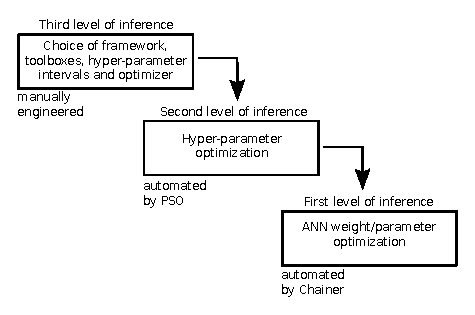
\includegraphics[width=0.7\columnwidth]{modeling/levels_of_opt.eps}
	\caption{The three levels of optimization and in how far they are automated}
	\label{fig:opt_levels}
\end{figure}

%PMSM
\textit{Escalante et. al.} performed an extensive model selection search via \gls{pso} and called it \gls{psms} \cite{EsMo2009}.
They achieved with this strategy high ranks in competitions by finding well-performing models in a full model search denoting a high-dimensional search space without over-fitting and simultaneously incorporating no prior knowledge of the domain.
Although their findings are based solely on binary classification tasks, chances are high, that model selection via \gls{pso} might also prove efficient for regression tasks.

\subsection{Particle Swarm Optimization}
\gls{pso}, originally proposed by \textit{Kennedy and Eberhart} in \cite{KeEb1995}, has its inspiration from natural clusters of biological entities showing individual and social behavior e.g. a bee hive, a school of fish or flocks of birds. Typically all members of the community share a common goal and they attempt to achieve it by exploring their environment individually while also reporting their findings to the society in order to support the overall course of exploration in investigating more promising areas.
The common exploration course is partially random but also slightly dragged to the better found solutions in an iterative manner.
A better site in the search space is defined with respect to a certain error measure representing an at least local optimum.
\gls{pso} is particularly popular because of its simple implementation and competitive performance in return, while computational cost is low as well.
One distinctive feature of \gls{pso} in comparison with evolutionary algorithms is the fact, that no selection is conducted.

The following formulations are based on \cite{Clerc2006}, which should be referred to in order to get a deep understanding of \gls{pso},
though \textit{Clerk's} explanations do not cover the application to hyper-parameters of \glspl{ann}.
The biological entity representatives are called \textit{particles} and all particles represent a \textit{swarm}.
Each particle has a position in the search space and a certain velocity during each time increment or iteration.
After every particle has evaluated the cost function at its position, these information is (partly) propagated through the swarm on which basis movement of each particle is updated.
Typically, the swarm stops after a predefined amount of iterations or until a target value for the cost function is found.
Depending on the update equation, it is also possible for the swarm to converge to a certain site in the search space due to decreasing velocities.

\subsubsection{Swarm Size}
In its simplest version, the number of particles, also called swarm size, is a fixed number.
While \textit{Clerc} states, that swarm sizes between 20 and 40 are sufficient for most problems, \textit{Escalante et. al.} has found during their \gls{psms} that smaller swarm sizes down to even five particles prove feasible \cite{Clerc2006, EsMo2009}.
However, the appropriate number of particles is task-dependent and one cannot infer from their investigations, that a small swarm  size would also be suitable for this thesis' particular task.
As mentioned before, optimizing the hyper-parameters of the hyper-parameter optimization itself (third level of inference) is outside the scope of this work and a swarm size of 100 particles throughout all investigations is applied instead.
Smaller amounts could lead to a global minimum as well, but with a view to the available hardware, which corresponds to a computing cluster, this large swarm size is indeed practicable in the sense of computing time and no risk of too less exploratory power must be taken.

\subsubsection{Initialization}
All particles are randomly initialized in the search space on the whole interval of each hyper-parameter.
Some are distributed uniformly while others are initialized geometrically, that is, randomly in the log domain.
The purpose behind geometrically distributed parameters is the fact, that they influence training in a multiplicative fashion and the same short adjustment has a bigger impact within smaller values than larger ones.

As of the very first iteration, each particle has its own velocity.
Thus, initial velocities are randomly distributed as well.
Distribution strategies are the same as for position initialization but with a bias in the interval towards zero in order to permit negative velocities as well.
The initialization interval for each particle's velocity per hyper-parameter is specifically
\begin{align}
	v_i\in[\frac{-(x_{max} - x_{min})}{2}, \frac{x_{max} - x_{min}}{2}],
\end{align}
with $v_i$ being the velocity of hyper-parameter $i$ and $x_{max}$ and $x_{min}$ denoting the upper and lower bound of the hyper-parameter's interval, respectively.

\subsubsection{Information and Informants}
The evaluation metric for a specific position in the hyper-parameter search space is chosen to be represented by the test set score.
Consequently, evaluating one spot in the search space is connected with the full training of a neural network and the following cross validation with the test set.
This is reasonable insofar, that a set of parameters is only interesting in terms of the resulting neural net's generalization abilities and, hence, the swarm should converge towards this objective.
The disadvantage of this procedure is the fact, that a spot's cost is not directly affected by the hyper-parameters explaining the search space but indirectly through the weights of the trained neural network, which were developed with a sense of randomness during training.
Moreover, the neural network weights are trained on the training set, selected with respect to the validation set performance and the test set score is in turn an independent performance measure.
This independence could give the swarm a blurred understanding of which sites are attractive and which are not.

Another point concerning swarm convergence is the specific implementation of ``social behavior'' or swarm intelligence.
One possible implementation would be the forwarding of each particle's best found position to every other particle such that each particle always knows what spot was the best up to the current iteration.
Nonetheless, this could lead to a biased convergence towards the initial positions and deaden the exploratory character of the swarm.
As an alternative, the global best position can be communicated to a certain particle by a group of informants composed of a number of other particles.
The group of informants for each particle varies randomly, in particular, each group of informants is made up by random other particles in the swarm to a predefined group size at each iteration.
This method resembles the spread of a rumor.
In \cite{Clerc2006} it has been shown, that, by this procedure and having always two informants, each particle has received information from almost definitely every other particle after ten iterations.
Thus, the number of random informants is set to two for all investigations.
Implementing this sort of communicating the global best position, the swarm is encouraged to explore the search space more thoroughly as not every particle acts according to the very same information.
Note, that the group of informants denotes a unidirectional information transfer, that implies, that if a particle knows a better spot than its informants, then they will not get to know that in turn.
In other words, the knowledge about the best global position a certain particle has been communicated to will only leave that particle to another, if that particle becomes an informant for another.

As soon as a spot is evaluated, the corresponding particle will overall hold following information:
\begin{itemize}
	\item its own position in the search space,
	\item this position's cost,
	\item the particle's best visited position in terms of lowest cost and the corresponding evaluation measure (\textit{personal best}) and
	\item the \textit{global best} position in the search space together with that spot's cost, as communicated by the particle's informants up to the current iteration.
\end{itemize}
In the beginning, each particle's personal best and global best is represented by its current position's cost.
If the particle's informants do not know a better site than the particle itself, the particle's global best remains unchanged.

\subsubsection{Velocity Update}
After each iteration, when all particle positions are evaluated, groups of informants are set and all information is transmitted, each particle's velocity is updated according to its current velocity, its personal best position and its global best position.
The update formulas per dimension are as follows:
\begin{align}
	v_i&\gets c_{self}v_i + c_{max}u(p_i - x_i) + c_{max}u(g_i - x_i)\\
	x_i&\gets x_i + v_i
\end{align}
where $x_i$ stands for the position in dimension $i$, $p_i$ and $g_i$ for personal best and global best position, respectively, while $u$ denotes a uniformly random value between $0$ and $1$.
The constant factor $c_{self}$ is similar to a momentum or the particle's confidence in its own velocity, whereas the constant $c_{max}$ represents the maximum confidence in its personal and global best position.
There are several alternatives to this approach imaginable.
Fig. \ref{fig:particle} illustrates how a particle's movement is affected by its displacement to its known personal and global best position.
\begin{figure}
	\centering
	\def\svgwidth{0.7\columnwidth}
         \import{eps/modeling/out/}{vel_update.pdf_tex}
         \caption{The basic displacement update for particles according to their best known sites}
         \label{fig:particle}
\end{figure}

Furthermore, the choice of the constant factors is made upon the recommendations in \cite{Clerc2006}, that are, $c_{self}= 0.7$ and $c_{max}= 1.43$.
These selections decrease velocities on average and the swarm is more likely to converge.

In addition, there is an off-bounds check in order to bring particles back to the hypercube defining the valid search space.
The heuristic here is to put the particle's position back to the upper or lower bound of the specific dimension that has been exceeded and to reset its velocity to zero.
Its subsequent velocity is then determined by its displacement to its personal and global best only, after which the particle would have an own velocity again.

The swarm is exploring the search space as long as the maximum number of iterations is not reached or until a predefined cost objective is found or until the swarm converges.
Here, the values are set to 100 iterations at maximum and a goal of less than \SI{1}{\kelvin\squared} in the \gls{mse} cost of the test score.
%What kind of PSO? Parametric or Non-Parametric(adaptive)? How many swarms?
%parallel computing rather than sequential, because one evaluation is long.

\subsection{Search Space}
In this work, the hyper-parameter search space consists of 15 dimensions, each limited to a specific predefined interval.
While continuous hyper-parameters, such as initial learn rate, are intuitively applied to the \gls{pso} search space, discrete parameters e.g. number of hidden layers and mutually exclusive choices as the optimizer technique need to be mapped onto a continuous interval coding in order to give a particle's velocity meaning there.

Tab. \ref{tab:hyperparams} shows an overview of the incorporated hyper-parameters.
Abbreviations for the hyper-parameter names are stated aside if given and are used during the remainder of the work for convenience.
Note, that some hyper-paramaters become active only in combination with certain choices in other hyper-parameters e.g. `PCA variance' has an effect only if `normalization' is set to `PCA'.

\begin{table}
	\rarray{1.3}
	\caption{A list of those hyper-parameters explaining the search space for the \gls{pso}}
	\label{tab:hyperparams}
	\centering
	\begin{tabular}{C{4.5cm} C{4cm} C{5cm}}
		\toprule
		hyper-parameter name & interval discretization & interval bounds/ choices\\
		\midrule
		architecture (arch)& mutually exclusive & \gls{lstm}, \gls{lstm} with peepholes or \gls{gru}\\
		number of hidden layers (n\_hl)& discrete & $[1, 3]$\\
		number of units per layer (n\_units)& discrete (log) & $[2, 256]$\\
		weight initialization - \quad distribution heuristic  & mutually exclusive & unit normal or uniform\\
		weight initialization - scaling heuristic & mutually exclusive & normalized or standard\\
		subsequence length (seq\_len)& discrete & $[30, 7880]$\\
		normalization (preprocess)& mutually exclusive & standard or \gls{pca}\\
		PCA variance (pca\_var)& continuous & $[0.5, 1.0]$\\
		lookback & discrete & $[0, 2000]$\\
		optimizer (opt)& mutually exclusive & \gls{adam}, Nesterov or \gls{sgd}\\
		initial learn rate (lr\_init) $\eta$& continuous (log) & $[1\cdot 10^{-4}, 1\cdot 10^{-1}]$\\
		learn rate decay factor (lr\_decay) $\alpha_d$ & continuous & $[0.5, 0.99]$\\
		regularization (active)& binary & $[0, 3]$\\
		gaussian noise $\sigma$ & continuous (log) & $[1\cdot 10^{-7}, 1\cdot 10^{-3}]$\\
		weight decay $\lambda$& continuous (log) & $[1\cdot 10^{-7}, 1\cdot 10^{-4}]$\\
		\bottomrule
	 \end{tabular}
\end{table}
The architecture parameter determines which memory block to choose (\gls{lstm}, with or without peepholes, or \gls{gru}; see sec. \ref{sec:arch}).

Number of hidden layers varies between one and three, while number of neurons per layer ranges from two to 256.
Intermediate experiments have been conducted with maximum number of layers at five and maximum number of units at 128, but the best models always certainly stayed at one layer and had their units near the upper bound such that these limits have been adjusted for the final experiments.
 
Weight initialization distribution and scaling were varied according to the heuristics explained in sec. \ref{ssec:init}.
The subsequence length is limited to at least 30 time-steps and at most the full length of the shortest profile in the training set.
Normalization was performed either with or without \gls{pca}, whose dimensionality reduction would have been utilized by keeping a variance between 50\% and 100\%.
The lookback parameter describes the amount of time-steps in the past, that are considered for enriching the input data with the first and second stochastic moments of each input parameter.
The selected optimizer was either \gls{adam}, Nesterov-style momentum or standard \gls{sgd}.
The initial learn rate is set geometrically, while learn rate decay is set uniformly.
The binary ``regularization'' parameter determines whether both, one or none of the two regularization techniques are applied.
In particular, ``zero'' equals to ``no regularization''; ``one'' to ``gaussian noise only''; ``two'' to ``weight decay only'' and ``three'' sets both regularization techniques active.
Gaussian noise on gradients has its standard deviation applied randomly while weight decay is determined by its penalty factor $\lambda$.

